\section{Residual Analysis}
\noindent\rule[\linienAbstand]{\linewidth}{\linienDickeDick}


\subsection{Introduction}
\noindent\rule[\linienAbstand]{\linewidth}{\linienDicke}
In our simple linear regression models we made the following assumptions:
\begin{enumerate}
  \item The relationship between response and the regressors is linear.
  \item The error $\varepsilon$ has mean zero.
  \item The error $\varepsilon$ has constant variance $\sigma^2$
  \item The errors are uncorrelated.
  \item The errors are normally distributed
\end{enumerate}
If some assumptions are violated we should be able to see them in the errors $\varepsilon_i$. On the other hand, the errors are unknown to us, so we have to deal with the residuals
\begin{equation}
  e_i = y_i - \hat{y}_i \;\;\;\text{for all}\;\;\; i \in {1,...,n}
\end{equation}
instead. The residuals are estimators of the random errors.\\

\textbf{Scaled Residuals}\\
If the errors are normally distributed, so are the residuals of a least-squares estimate. Since the variance of the residuals depends on $x_0$ it is not equal to the variance of the errors. Therefore we use scaled residuals
\begin{equation}
  \tilde{e}_i = \frac{e_i}{\sqrt{1 - \left(\frac{1}{n} + \frac{(x_i - \bar{x})^2}{S_{xx}}\right)}} \;\;\;\text{for all}\;\;\; i \in {1,...,n}
\end{equation}


\textbf{Coefficient of Determination}\\
The coefficient of determination is a measure of the linear relationship between the response variable and the fit.\\

In simple linear regression with only one explanatory variable the coefficient of determination is defined by
\begin{equation}
  R^2 = \frac{SS_{\textup{fit}}}{S_{yy}}
\end{equation}
where
\begin{equation}
  \begin{split}
    SS_{\textup{fit}} &= \sum_{i=1}^n(\hat{y}_i - \bar{\hat{y}}_i)^2 = \hat{\beta}_1^2 S_{xx}\\
    SS_{yy} &= \sum_{i=1}^n(y_i - \bar{y}_i)^2
  \end{split}
\end{equation}
Therefore the coefficient of determination is
\begin{equation}
  R^2 = \hat{\beta}_1^2 \frac{S_{xx}}{S_{yy}} = \frac{S_{xy}^2}{S_{xx} S_{yy}} = \textup{Cor}(x, y)^2
\end{equation}

In multiple regression and simple linear regression with at least one explanatory variable the coefficient of determination is identical to the squared correlation between the response variable $y$ and the fitted values $\hat{y}$
\begin{equation}
  R^2 = \textup{Cor}(y, \hat{y})^2 = \frac{S_{y\hat{y}}^2}{S_{yy} S_{\hat{y}\hat{y}}}
\end{equation}

The coefficient of determination is a global measure for the goodness of fit and it says nothing about the suitability of the regression model.

\subsection{Diagnostic Tools}
\noindent\rule[\linienAbstand]{\linewidth}{\linienDicke}
What follows is a description of three graphical diagnostic tools to check model assumptions 1, 2, 3 and 5. The aim is to be sure that there are no dangerous discrepancies from the assumptions in the data. All three tools are based on the residuals which are representations of the unknown errors.\\

\textbf{Tukey-Anscombe Plot}\\
The idea of this plot is to plot residuals $e_i$ versus fitted values $\hat{y}_i$.
With the Tukey-Anscombe Plot we can check whether the second model assumption holds true.\\
Residuals in any interval of the Tukey-Anscombe plot should vary randomly around the horizontal line at zero.

\begin{table}[H]
  \setlength{\tabcolsep}{0.2em}
  \scriptsize
  \begin{tabular}{p{\linewidth / 2 - 0.5em}@{\hskip 1em}p{\linewidth / 2 - 0.5em}}
    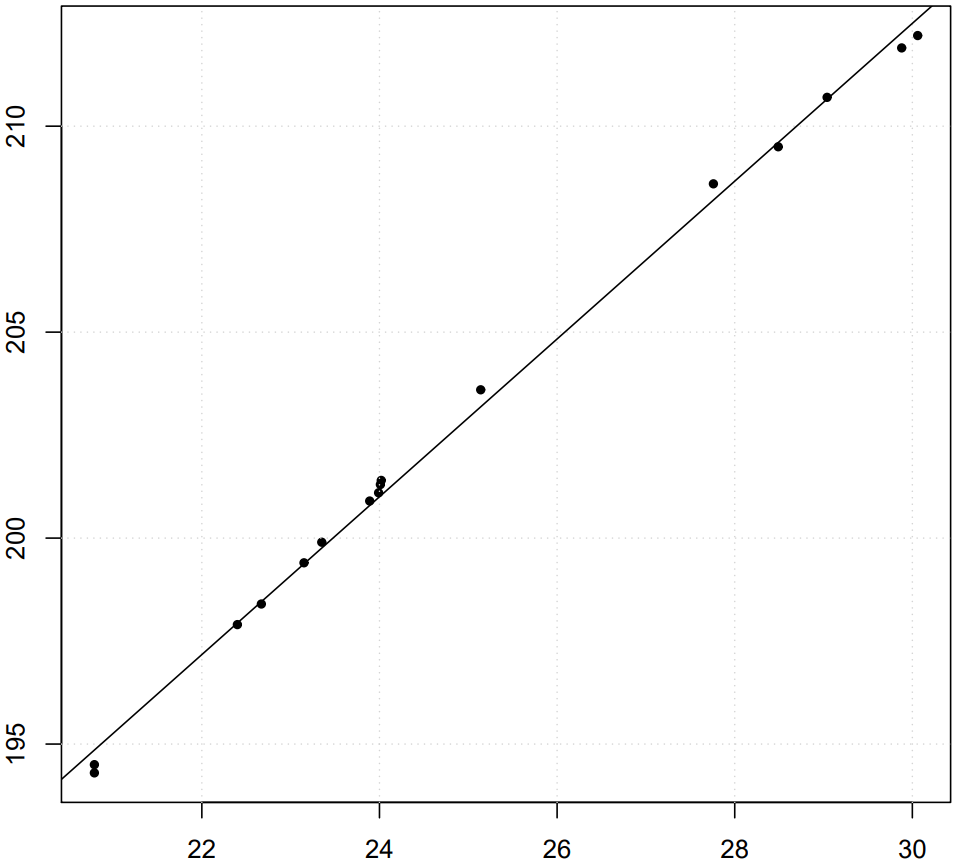
\includegraphics[width=\linewidth]{Pics/8.2.1.png}& 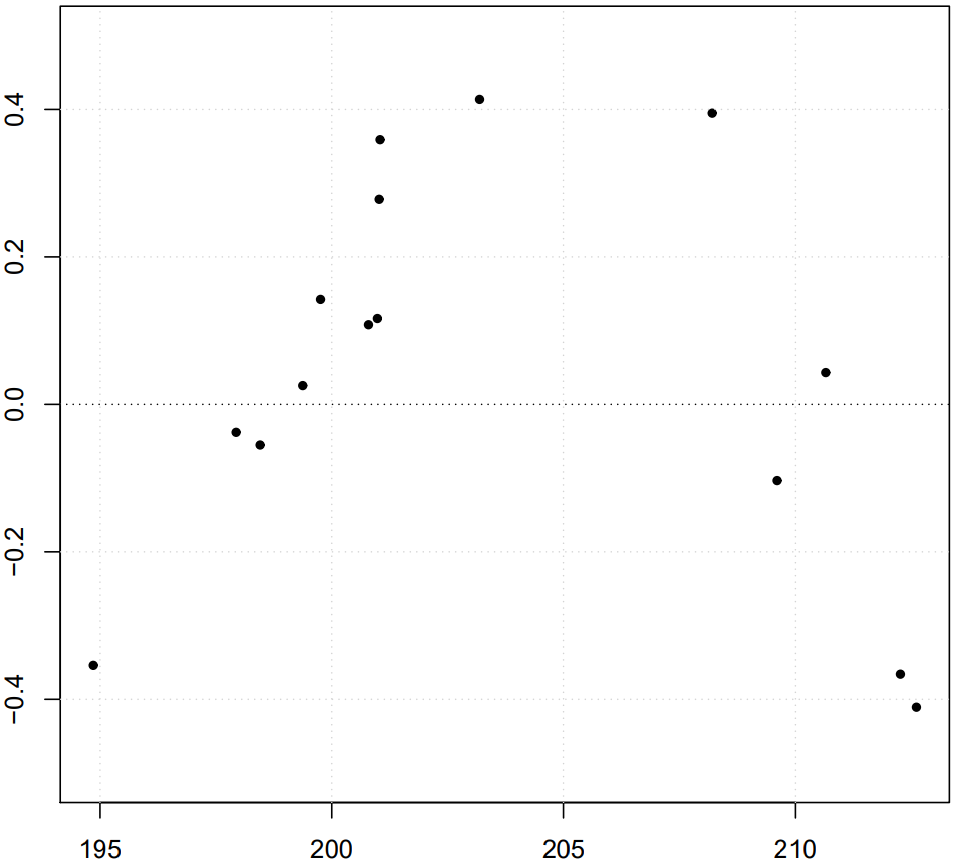
\includegraphics[width=\linewidth]{Pics/8.2.2.png} \\
    Best linear model &
    Tukey-Anscombe plot of the model. The points are not spread uniformly around the horizontal line indicating a bad model.\\
  \end{tabular}
\end{table}

Model assumption number two states that the errors should have mean zero. To check this assumption it is best to smooth the data in the
Tukey-Anscombe plot. We are still left with the question: Is such a curved curve due to chance possible? An informal method to find answers is based on bootstrap simulations\\

\textbf{Bootstrap Simulation}\\
What follows is a briev explanation of the bootstrap simulation:\\
- Calculate the best linear model with $\textup{Var} = \hat{\sigma}^2$ and calculate the smooth curve of the residuals.\\
- Simulate new observations based off the fitted model.
- Calculate the smooth residuals of the simulated obervation and add it to the diagram.\\
- Repeat 19 times. (1 + 19 observations)
\begin{table}[H]
  \setlength{\tabcolsep}{0.2em}
  \scriptsize
  \begin{tabular}{p{\linewidth / 2 - 0.5em}@{\hskip 1em}p{\linewidth / 2 - 0.5em}}
    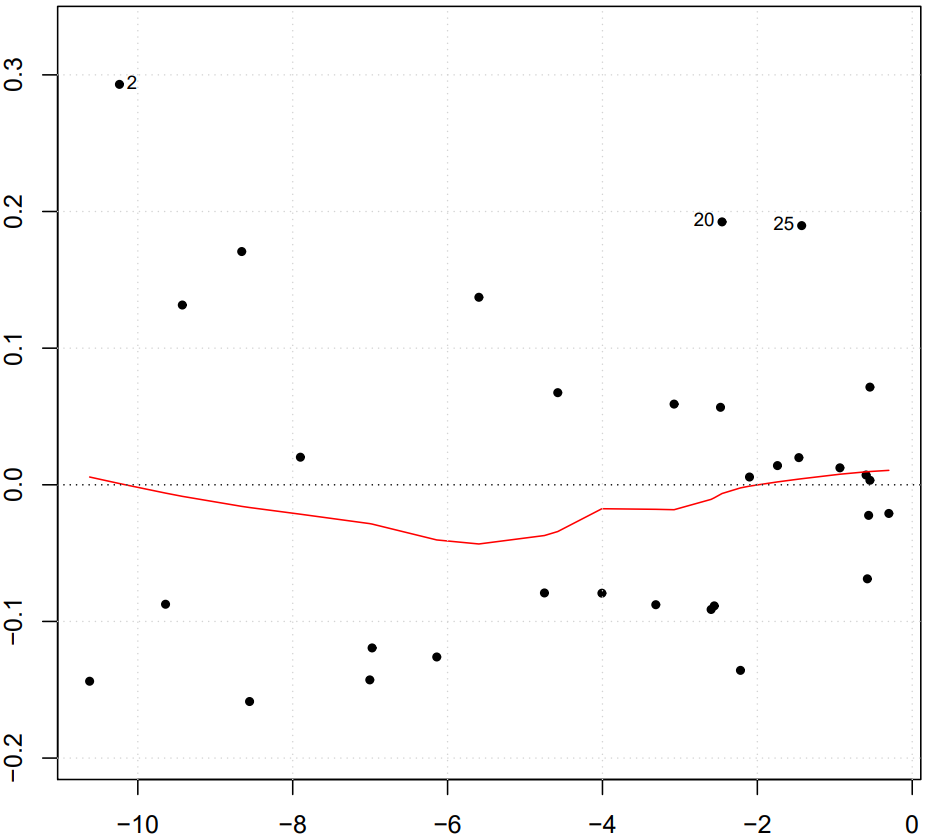
\includegraphics[width=\linewidth]{Pics/8.2.5.png}& 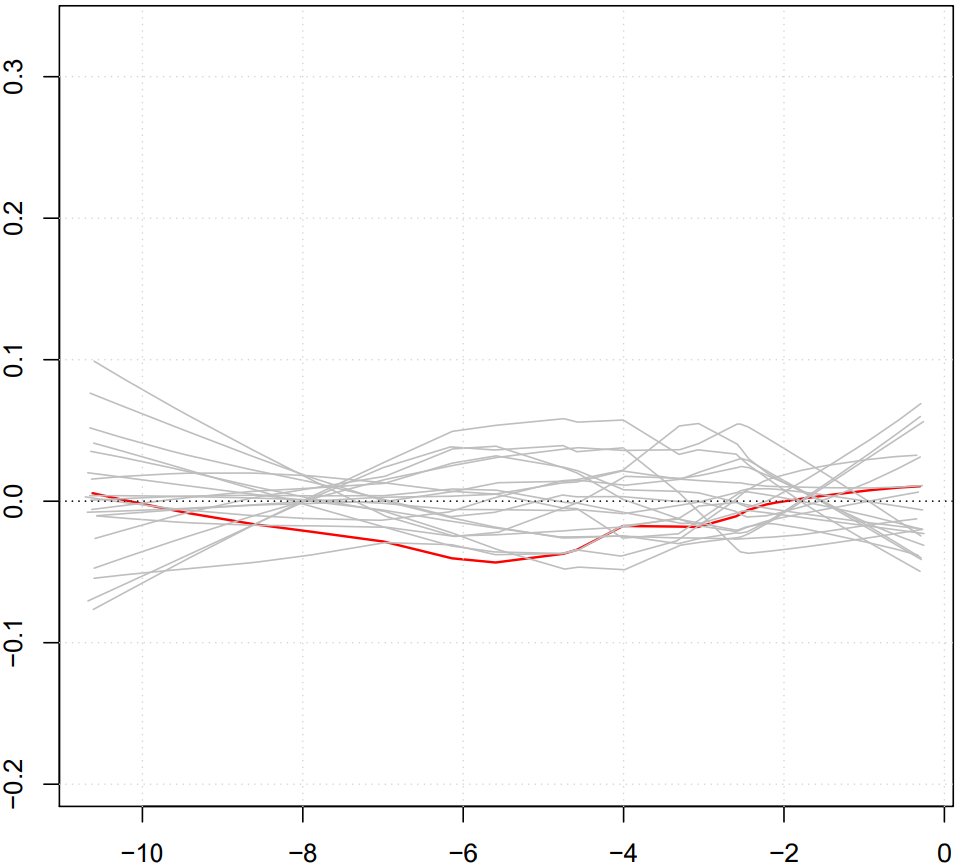
\includegraphics[width=\linewidth]{Pics/8.2.6.png} \\
    Tukey-Anscombe plot with smoothed residuals (red). The smoothed curve shows a clear curvature (which is bad). &
    Tukey-Anscombe plot with 19 simulated smoothed residuals (gray). The curved smooth curve is not an extreme curve among all 20. We conclude that the model fits the data.\\
  \end{tabular}
\end{table}

\textbf{Scale-Location Plot}\\
The idea of this plot is to plot the residuals of square-root of absolute standardised residuals $\sqrt{|\tilde{e}_{std, i}|}$ versus fitted values $\hat{y}_i$. With the scale-location plot we can check whether the third model assumption holds true.\\
If the smoothed curve of square-root of the absolute standardised residuals is approximately horizontal, then the errors have equal variance.
\begin{table}[H]
  \setlength{\tabcolsep}{0.2em}
  \scriptsize
  \begin{tabular}{p{\linewidth / 2 - 0.5em}@{\hskip 1em}p{\linewidth / 2 - 0.5em}}
    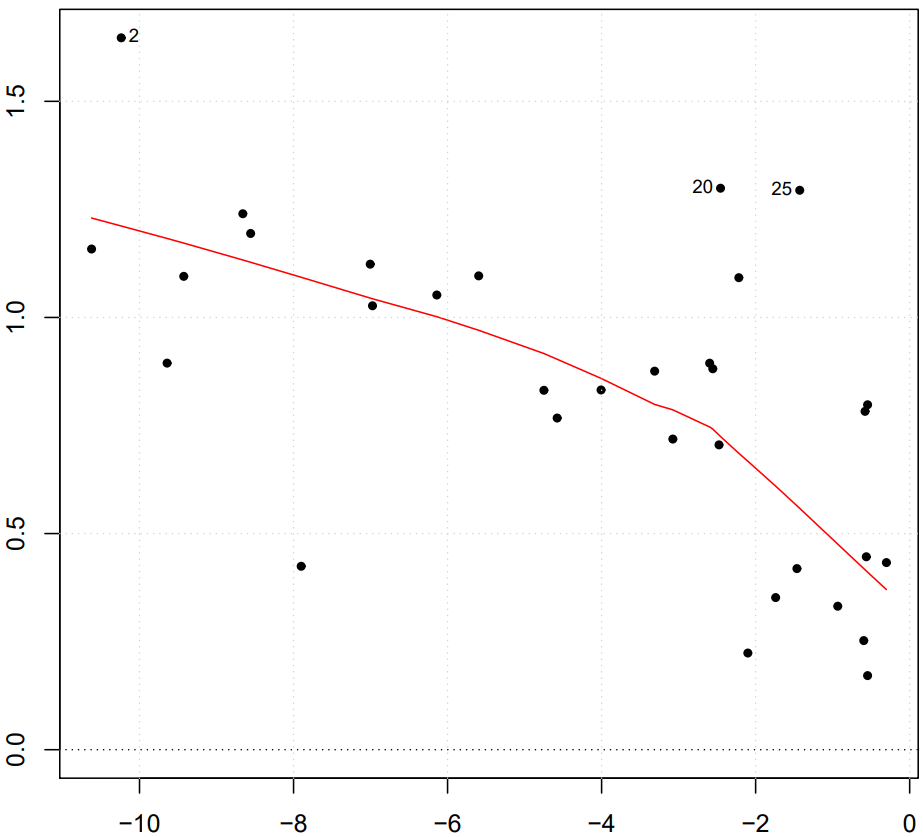
\includegraphics[width=\linewidth]{Pics/8.2.7.png}& 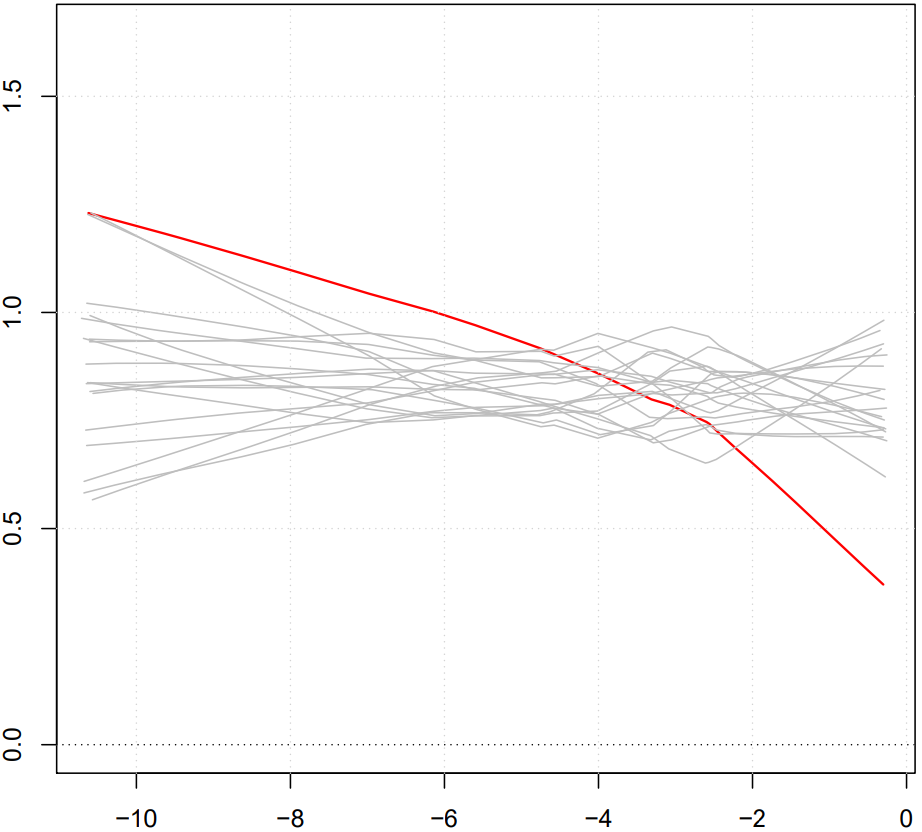
\includegraphics[width=\linewidth]{Pics/8.2.8.png} \\
    Scale-location plot with smoothed residuals (red). We observe a clear downward trend in residual scattering. &
    Scale-location plot with 19 simulated smoothed residuals (gray). The simulation confirms the extraordinary behavior.\\
  \end{tabular}
\end{table}

\textbf{Normal q-q Plot (and Histogram)}\\
The idea of the histogram is to compare histogram of residuals $e_i$ with normal density function with parameters $0$ and $\hat{\sigma}^2$. It is often difficult to compare a histogram with a bell shaped curve and the histogram is very sensitive to the number of histogram cells and the breakpoints between cells.\\
The idea of the normal q-q plot is to plot quantiles of the empirical distribution of the of the standardised residuals $\tilde{e}_{std, i}$ versus quantiles of the normal distribution.\\
If the data is from a normal distribution, the points in the q-q plot scatter around a straight line.

\begin{table}[H]
  \setlength{\tabcolsep}{0.2em}
  \scriptsize
  \begin{tabular}{p{\linewidth / 2 - 0.5em}@{\hskip 1em}p{\linewidth / 2 - 0.5em}}
    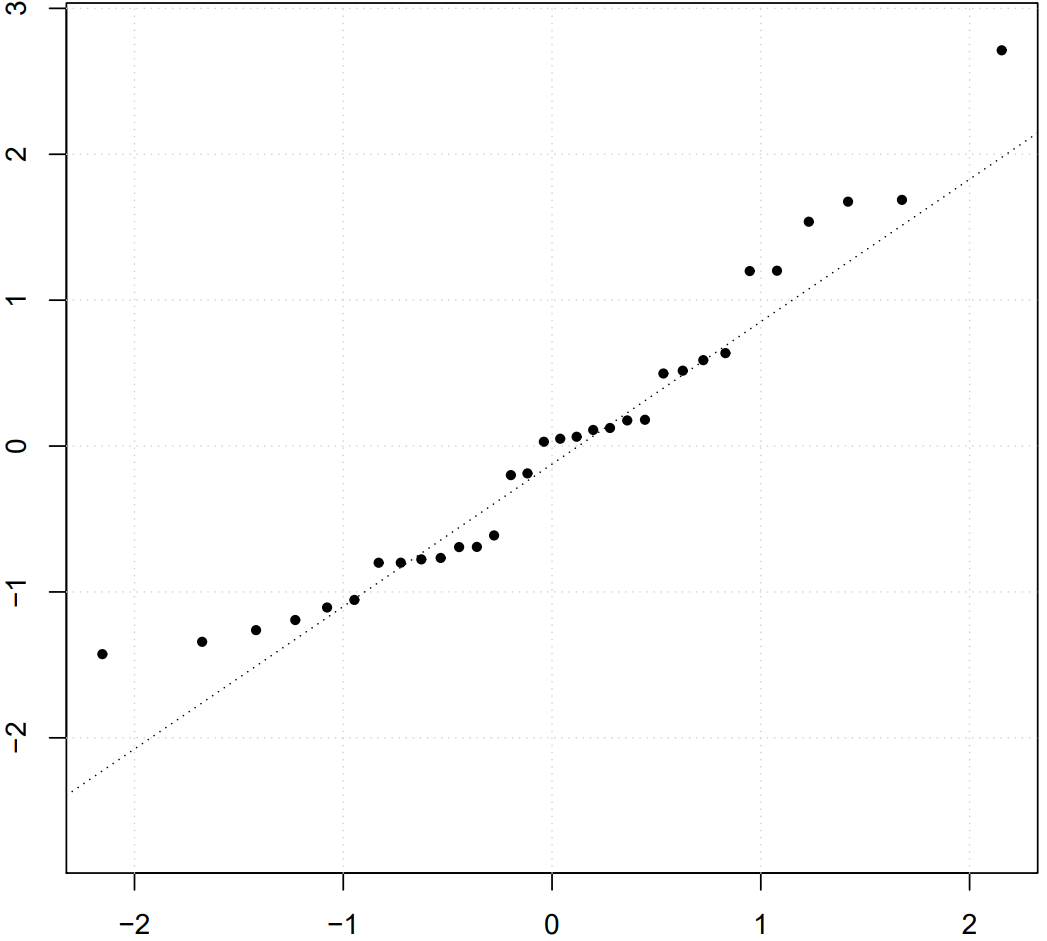
\includegraphics[width=\linewidth]{Pics/8.2.10.png}& 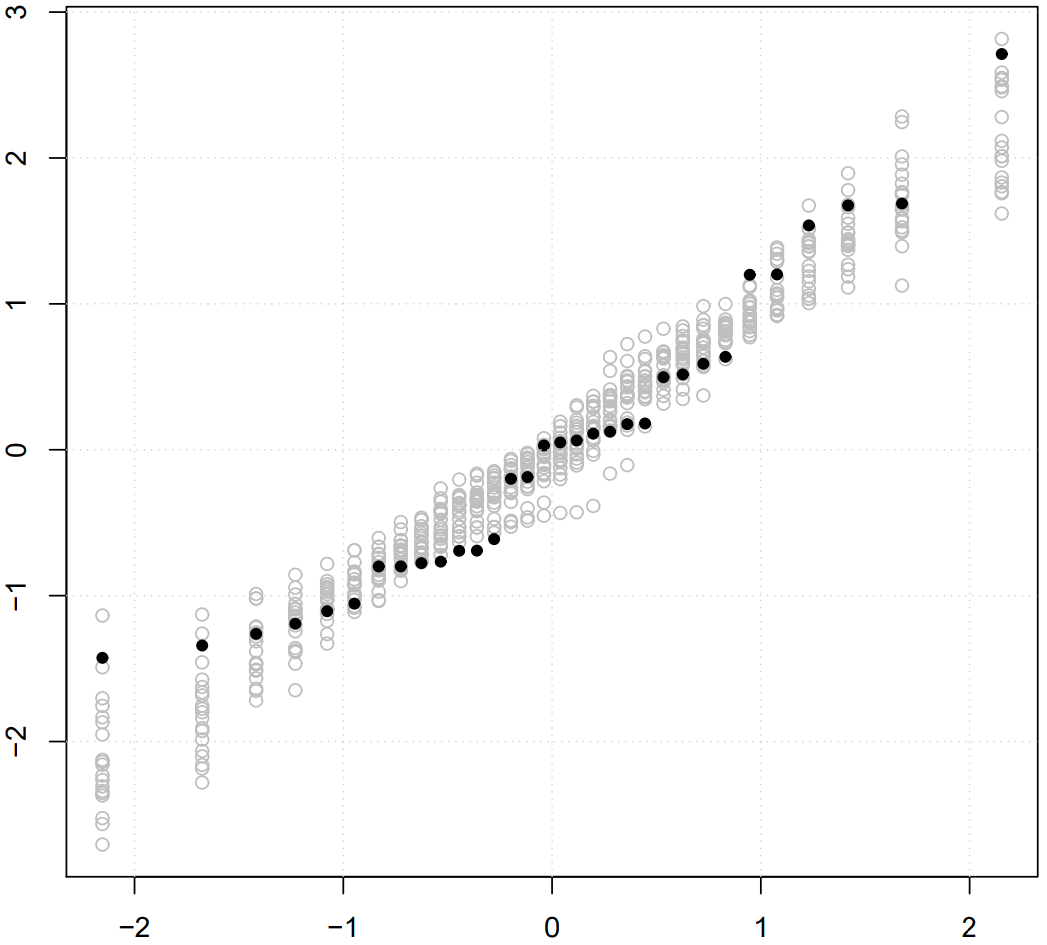
\includegraphics[width=\linewidth]{Pics/8.2.11.png} \\
    q-q plot with standardised residuals. We can observe a discrepancy to normality &
    q-q plot with 19 simulated standardised residuals (gray). The simulation shows us that this discrepancy might be due to random fluctuations\\
  \end{tabular}
\end{table}
